\chapter{評価手法と結果}
\label{chap:evaluation}
\section{本提案の評価概要}
本章では\ref{chap:implementation_and_experimentation}章で
述べたシミュレーションにおける結果についてまとめる.

\ref{section:要件1に対するシミュレーション結果}節では
\ref{section:要件1}で述べた配送遅延の増加防止の効果について, 
\ref{section:2030年代の地球・月間を想定したシミュレーションのシナリオとパラメータ}節で述べた
地球-月間のシミュレーション, 
\ref{section:2040年代の地球・月・火星間を想定したシミュレーションのシナリオとパラメータ}節で述べた
地球-火星間の距離に応じた3種類のシミュレーションにおける
配送を試みたBundleの到達率とその平均遅延を示す. 

\ref{section:要件2に対する更新メッセージによるリンク消費}節では
\ref{section:要件2}で述べた運用面での効果について, 
上記それぞれのシミュレーションについて, 
運用上のデメリットとして天体間でCPUPコマンドがどれだけリンク消費をするかを示す. 



\section{要件1に対するシミュレーション結果}
\label{section:要件1に対するシミュレーション結果}
\ref{section:2030年代の地球・月間を想定したシミュレーションのシナリオとパラメータ}節で述べた
地球-月間のシミュレーションおよび, 
\ref{section:2040年代の地球・月・火星間を想定したシミュレーションのシナリオとパラメータ}節で述べた
地球-火星間の距離に応じた3種類のシミュレーションにおける
配送を試みたBundleの到達率とその平均遅延は以下のようになった. 

%地球・月間のシミュレーション結果

\begin{figure}[tbh]
    \centering
    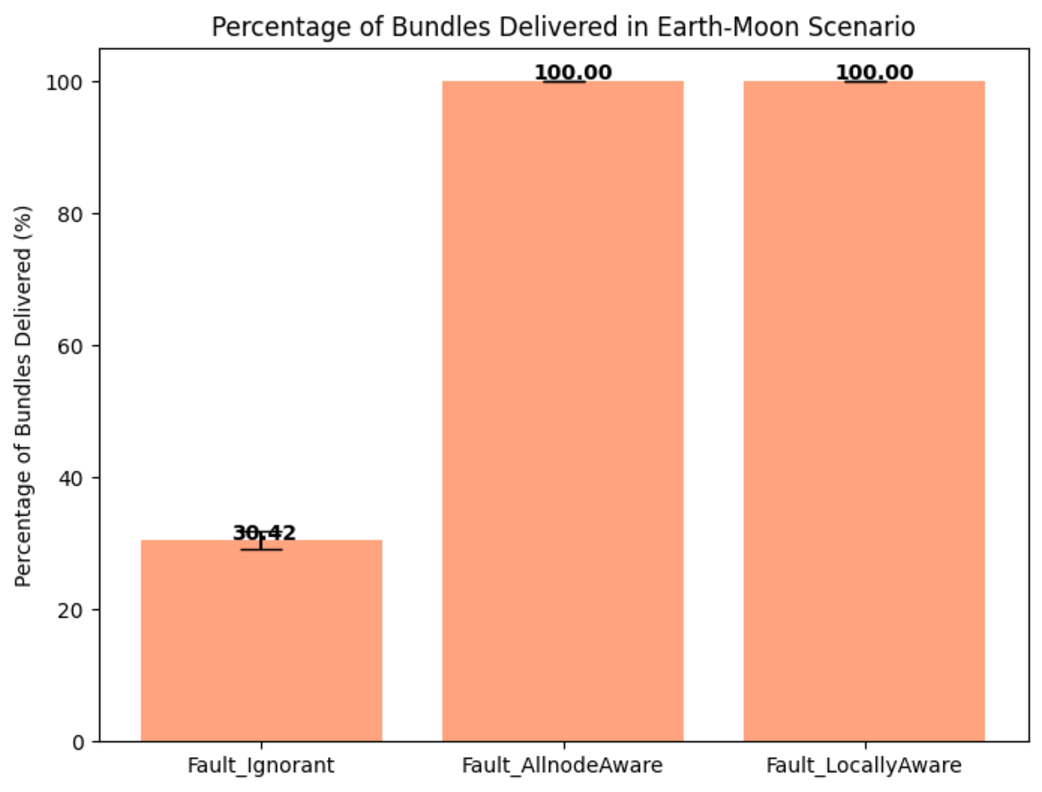
\includegraphics[width=0.7\textheight]{results/moon/moon_bundle.pdf}
    \caption{地球・月間シナリオにおけるバンドルの到達率}
    \label{fig:graph_bundle_earth_moon}
    \begin{minipage}{\textwidth}
        \centering
        \vspace{3mm}
        地球・月間シナリオにおけるノード6に向けたBundleの到達率
    \end{minipage}
\end{figure}

\begin{figure}[tbh]
    \centering
    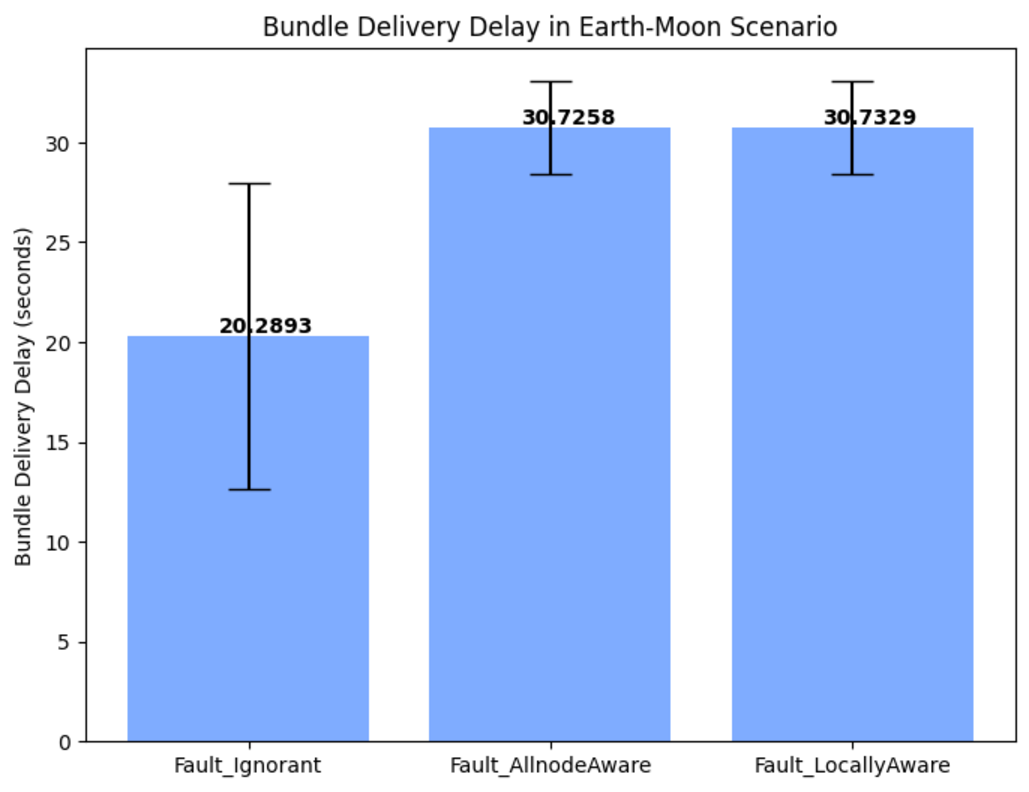
\includegraphics[width=0.7\textheight]{results/moon/moon_delay.pdf}
    \caption{地球・月間シナリオにおけるバンドルの到達遅延}
    \label{fig:graph_delay_earth_moon}
    \begin{minipage}{\textwidth}
        \centering
        \vspace{3mm}
        地球・月間シナリオにおけるノード6に向けたBundleの到達遅延
    \end{minipage}
\end{figure}

%地球・火星間のシミュレーション結果
\begin{figure}[tbh]
    \centering
    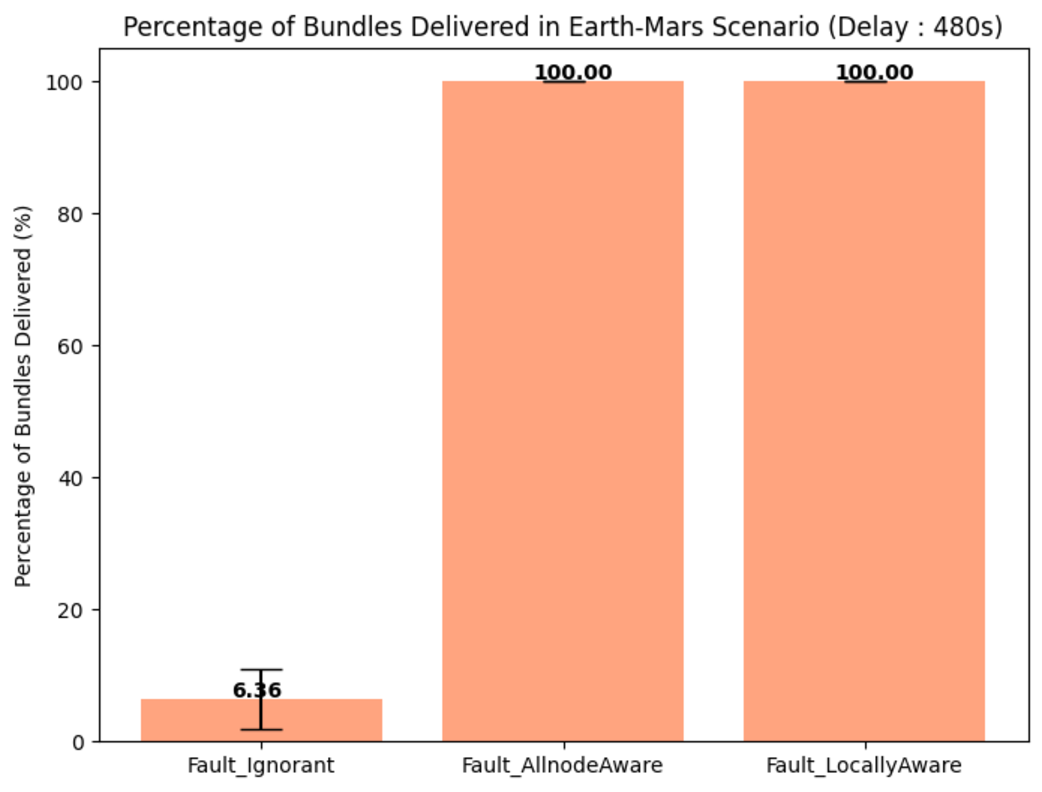
\includegraphics[width=0.7\textheight]{results/mars_distance_480/mars_480_bundle.pdf}
    \caption{地球・火星間シナリオ(距離480光秒)におけるバンドルの到達率}
    \label{fig:graph_bundle_earth_mars_480}
    \begin{minipage}{\textwidth}
        \centering
        \vspace{3mm}
        地球・火星間シナリオ(距離480光秒)におけるノード6に向けたBundleの到達率
    \end{minipage}
\end{figure}

\begin{figure}[tbh]
    \centering
    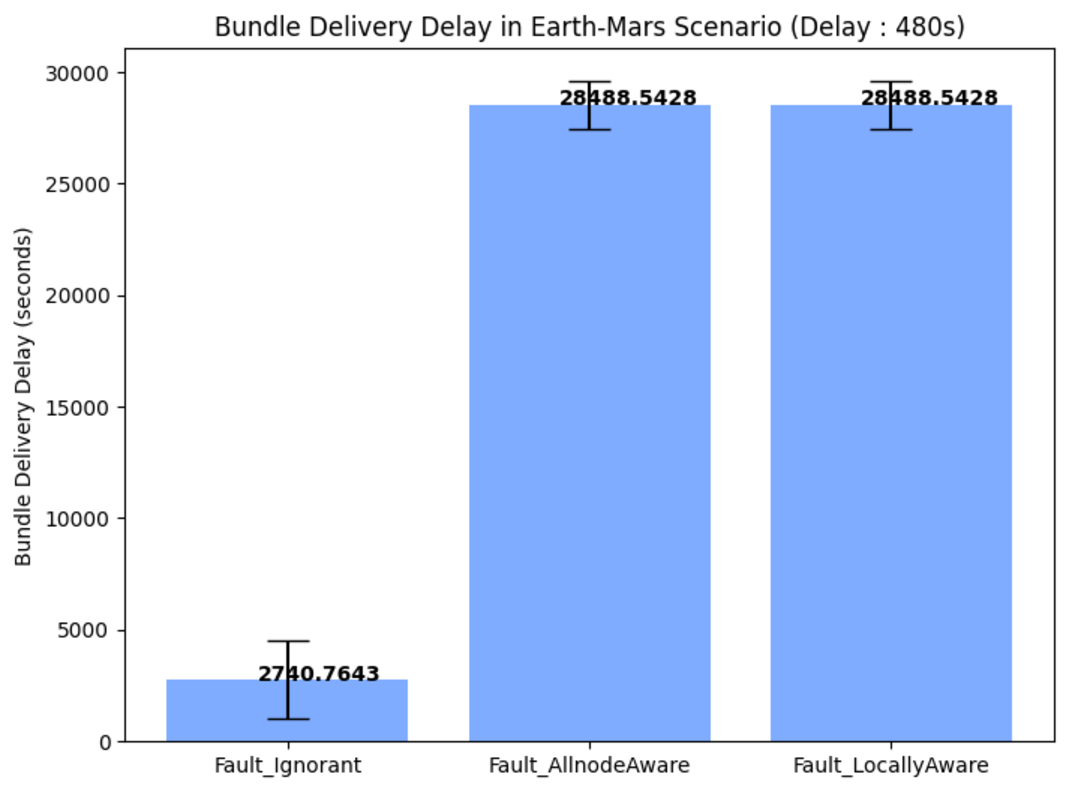
\includegraphics[width=0.7\textheight]{results/mars_distance_480/mars_480_delay.pdf}
    \caption{地球・火星間シナリオ(距離480光秒)におけるバンドルの到達遅延}
    \label{fig:graph_delay_earth_mars_480}
    \begin{minipage}{\textwidth}
        \centering
        \vspace{3mm}
        地球・火星間シナリオ(距離480光秒)におけるノード6に向けたBundleの到達遅延
    \end{minipage}
\end{figure}

\begin{figure}[tbh]
    \centering
    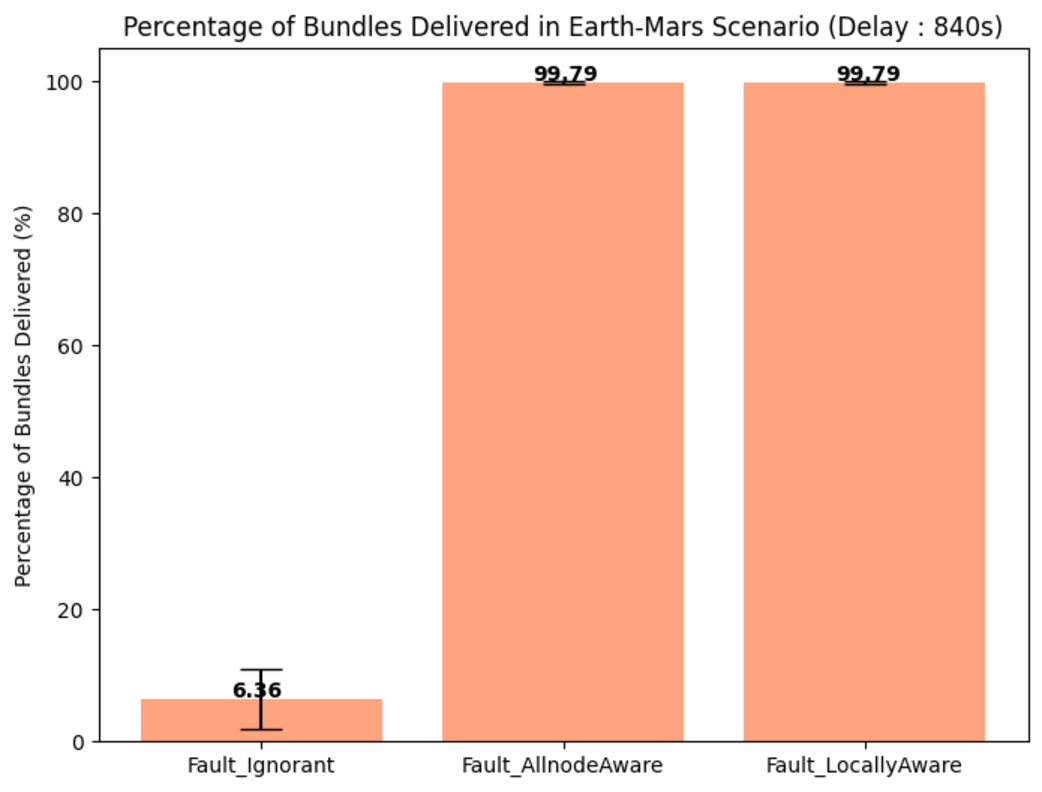
\includegraphics[width=0.7\textheight]{results/mars_distance_840/mars_840_bundle.pdf}
    \caption{地球・火星間シナリオ(距離840光秒)におけるバンドルの到達率}
    \label{fig:graph_bundle_earth_mars_840}
    \begin{minipage}{\textwidth}
        \centering
        \vspace{3mm}
        地球・火星間シナリオ(距離840光秒)におけるノード6に向けたBundleの到達率
    \end{minipage}
\end{figure}

\begin{figure}[tbh]
    \centering
    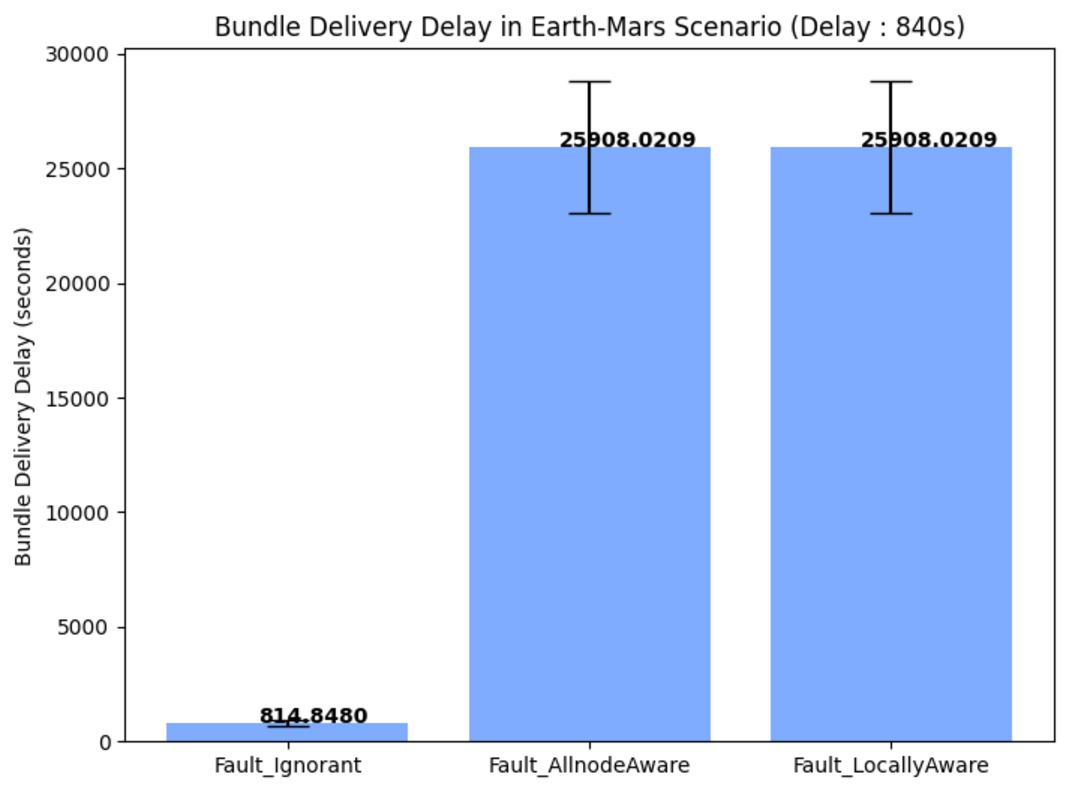
\includegraphics[width=0.7\textheight]{results/mars_distance_840/mars_840_delay.pdf}
    \caption{地球・火星間シナリオ(距離840光秒)におけるバンドルの到達遅延}
    \label{fig:graph_delay_earth_mars_840}
    \begin{minipage}{\textwidth}
        \centering
        \vspace{3mm}
        地球・火星間シナリオ(距離840光秒)におけるノード6に向けたBundleの到達遅延
    \end{minipage}
\end{figure}

\begin{figure}[tbh]
    \centering
    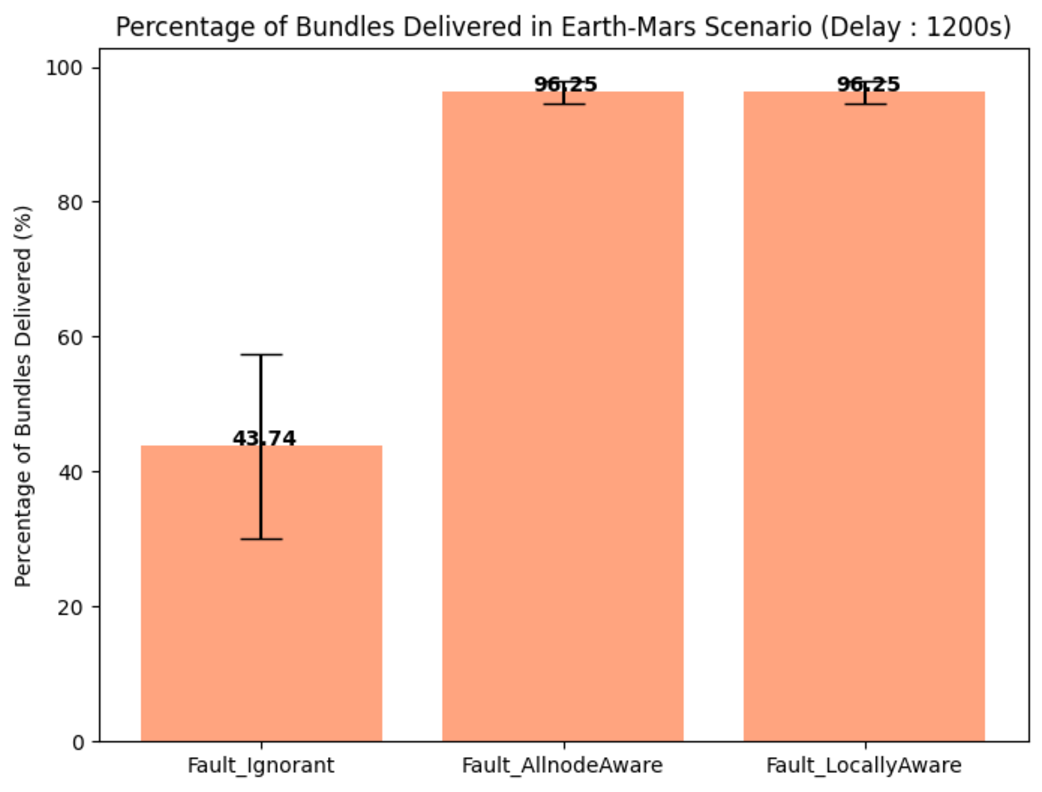
\includegraphics[width=0.7\textheight]{results/mars_distance_1200/mars_1200_bundle.pdf}
    \caption{地球・火星間シナリオ(距離1200光秒)におけるバンドルの到達率}
    \label{fig:graph_bundle_earth_mars_1200}
    \begin{minipage}{\textwidth}
        \centering
        \vspace{3mm}
        地球・火星間シナリオ(距離1200光秒)におけるノード6に向けたBundleの到達率
    \end{minipage}
\end{figure}

\begin{figure}[tbh]
    \centering
    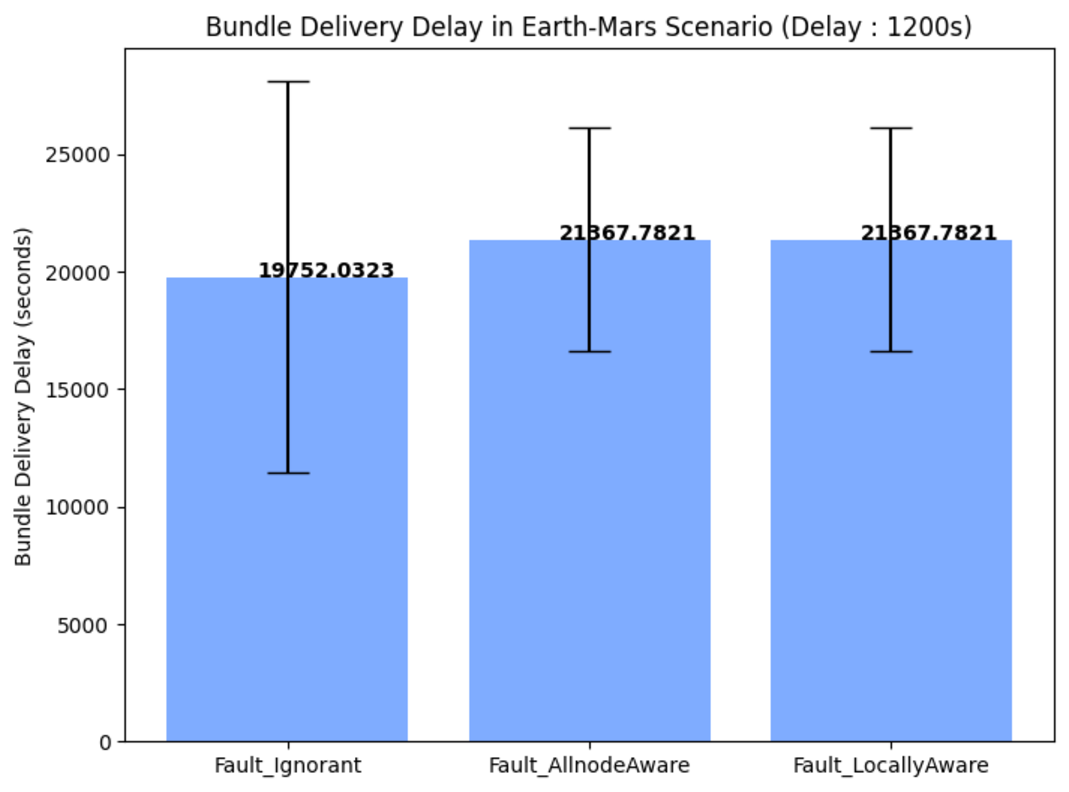
\includegraphics[width=0.7\textheight]{results/mars_distance_1200/mars_1200_delay.pdf}
    \caption{地球・火星間シナリオ(距離1200光秒)におけるバンドルの到達遅延}
    \label{fig:graph_delay_earth_mars_1200}
    \begin{minipage}{\textwidth}
        \centering
        \vspace{3mm}
        地球・火星間シナリオ(距離1200光秒)におけるノード6に向けたBundleの到達遅延
    \end{minipage}
\end{figure}


\section{要件2に対する更新メッセージによるリンク消費}
\label{section:要件2に対する更新メッセージによるリンク消費}
\ref{section:要件2}で述べたように, 既存手法では天体間での更新メッセージの送信が必要であり, 
その際にリンクを消費する. 一方, 本提案手法では自天体内のノードにのみ更新メッセージを送信するため, 
そのメッセージによる天体間リンクの消費は一切ない. 
本論文では表\ref{table:cpup_pdu_format}および表\ref{table:command_block_format}で示した
CPUPのPDUとその中のCommand Blockについては先行研究で用いられたフォーマットをそのまま用いることを想定する. 
1回のContact失敗とそれを知らせる更新のメッセージが単一のBundleで送信される場合, 
Command Blockは以下のようになることが想定される. 


\begin{table}[htbp]
    \centering
    \label{table:delete_command_block_format}
    \begin{tabular}{|c|c|c|c|}
        \hline
        Byte 0 & Byte 1 & Byte 2 & Byte 3 \\
        \hline
        \multicolumn{1}{|c|}{Version num.} & \multicolumn{3}{c|}{Number of Command Blocks (SDNV)} \\
        Byte 4 & Byte 5 & Byte 6 & Byte 7  \\
        \hline
        \multicolumn{2}{|c|}{Creation Timestamp (SDNV)} & \multicolumn{2}{c|}{Command Expiry (SDNV)} \\
        \hline
        Byte 8 & Byte 9 & Byte 10 & Byte 11 \\
        \hline
        \multicolumn{3}{|c|}{Command Originator (SDNV)} & Command Type \\
        \hline
        Byte 12 & Byte 13 & Byte 14 & Byte 15 \\
        \hline
        \multicolumn{4}{|c|}{ID of Contact to delete} \\
        \hline
    \end{tabular}
    \caption{既存手法における単一のContactを削除するCPUPのCommand Block}
    \begin{minipage}{\textwidth}
        \centering
        \vspace{3mm}
    \end{minipage}
  \end{table}

リンク消費量は以下のようになる. 

\begin{equation}
    \text{リンク消費量} = \text{CPUPのPDUのサイズ} \times \text{削除するContact数}
\end{equation}

\ref{section:2030年代の地球・月間を想定したシミュレーションのシナリオとパラメータ}節で述べた地球-月間のシナリオにおいては, 
生成した480回のContactのうち100回のContactを失敗させるシナリオであるため, リンク消費量は以下のようになる. 

\begin{equation}
    \text{リンク消費量} = 8 \times 100 = 800
\end{equation}
